\chapter{Desarrollo}\label{cha:solucion}
% AÑADIR UNA INTRODUCCIÓN A LA SOLUCIÓN

\section{Arquitectura del sistema}\label{section:arquitecturaSistema}
A grandes rasgos, existe en el medio del sistema una aplicación en la nube denominada \emph{Nube de Conductores} que se encarga de hacer llegar los mensajes procedentes de los ciclistas a los vehículos a motor, y los mensajes enviados por los vehículos a motor a los ciclistas. En la figura \ref{fig:ArquitecturaSistema} se puede observar de qué elementos está compuesto el sistema y cómo se comunican entre ellos.

Los vehículos a motor no se comunican directamente con la \emph{Nube de Conductores}, sino que utilizan un dispositivo OBU para mandar mensajes a una unidad desplegada en carretera llamada RSU. Esta última recoge los mensajes que escucha a través de Broadcast y los reenvía a la nube por conectividad 3G.

Por otro lado, los ciclistas envían información a la \emph{Nube de Conductores} a través de 3G o 4G; dependiendo de la disponibilidad. \'Estos también pueden agruparse empleando \emph{Wi-Fi 802.11} mediante la creación de un \emph{HUB} de dispositivos móviles, en el cual se envían notificaciones sobre los eventos que aparezcan.

\begin{figure}[H]
	\begin{center}
		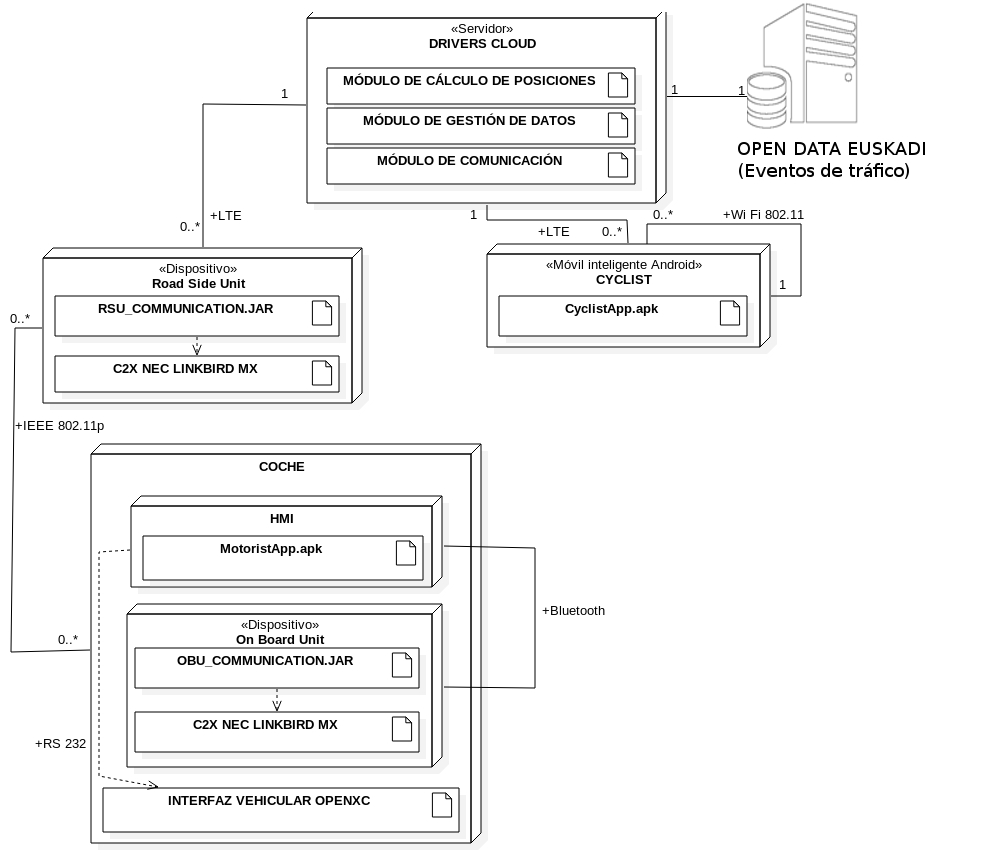
\includegraphics[scale=0.4]{arquitectura_global}
		\caption{Arquitectura del sistema}
		\label{fig:ArquitecturaSistema}
	 \end{center}
\end{figure}

\section{Nube de Conductores}\label{section:NubeConductores}
El núcleo del sistema es una aplicación desplegada en la nube, la cual se ha denominado \emph{Nube de Conductores}, donde se concentran en una base de datos la información relativa a ciclistas y vehículos a motor. Un servicio de aplicación web embebido llamado \emph{Jetty} se encarga de recibir y atender los mensajes \emph{HTTP/1.1} que son enviados desde la parte de vehículos a motor y ciclistas. Dos \emph{Handler} independientes se encargan de filtrar los mensajes que no han sido correctamente construidos, es decir, tienen un formato inválido, e insertar y actualizar los datos de la base de datos.

Para el despliegue de la aplicación se utilizado una máquina virtual \emph{Ubuntu Server 14.04 LTS} que cuenta con 2048 MiB de memoria RAM y 2 n\'cleos para procesamiento. También se ha reservado un dominio público para que las peticiones puedan ser enviadas al servidor. Gracias a la herramienta \emph{ANT} se puede cambiar fácilmente la plataforma donde se distribuya la aplicación, además esta configurada para poder ser ejecutada directamente con el comando \emph{run}.

% AÑADIR UN DIAGRAMA DE CLASES EXPLICATIVA DE LA COMUNICACIÓN ENTRANTE Y SALIENTE DE LA NUBE

\subsection{Comunicación entre plataformas}\label{ssection:comunicacion_plataformas}
La conexión entre la parte de los vehículos a motor y de los ciclistas hacia la nube se establece a través de tecnología móvil Long Term Evolution (LTE) o Third Generation (3G), dependiendo de la disponibilidad, aunque la manera de comunicarse con la \emph{Nube de Conductores} es diferente. La Nube de Conductores actúa como intermediario entre las aplicaciones desarrolladas en el lado de los motoristas y el de los ciclistas.

% AÑADIR REFERENCIAS A LAS SECCIONES DE CICLISTAS Y VEHÍCULOS A MOTOR
\subsubsection{Mensajes a ciclistas}\label{sssection:mensajes_ciclistas}
Se ha desarrollado una aplicación \emph{Android} desde la cual se manda a la nube actualizaciones sobre la posición del usuario o el grupo que el usuario haya creado. \'Este recibe notificaciones sobre las posiciones de los vehículos próximos, y otros diferentes eventos que pueden darse en la carretera; por ejemplo, un accidente de tráfico. Se ha contemplado la posibilidad de salidas en grupo de ciclistas, para ello se ha habilitado una modalidad específica mediante la cual se crea un grupo que se comunica entre sus miembros a través de una red privada \emph{Wi-Fi 802.11}. Los diferentes miembros se mantienen actualizados sobre los diferentes eventos a través de un nodo denominado líder, el cual es el enlace a la nube tanto para reportar la posición del grupo de ciclistas como para recibir mensajes de la nube y retransmitir éstos al resto de miembros.

Para comunicarse con los dispositivos Android se requiere un sistema de comunicación por el cual aunque los ciclistas no tengan en un momento determinado cobertura, los mensajes no se pierdan. Se ha elegido la plataforma Google Cloud Messaging (GCM), la cual se encarga de gestionar que los mensajes lleguen al destino aunque éste se encuentre temporalmente inaccesible mediante tecnología \emph{Push} [\ref{alg:gcmFuncionamientoMensajes}]. 

El mensaje debe respetar el formato que la API de GCM indica y puede observarse en el algoritmo \ref{alg:gcmformato}, donde \emph{ID\_ANDROID} es el identificador del dispositivo Android al que se le va a enviar el mensaje, y \emph{DATOS} un objeto \emph{JSON} con la información se que desea enviar. Para crear un identificador único, se puede emplear el que crea Android cuando se introduce la cuenta de correo personal en el móvil. El identificador de Android está formada por una cadena hexadecimal de 64 bit, la cual es poco probable que se repita. En el caso de que se quisiese reducir aún más la probabilidad de repetición, se puede mezclar el identificador de Android con el que la compañía de telefonía emplea para identificar nuestro dispositivo; aunque esto último aumenta el tamaño de los mensajes.

\begin{listing}
	\begin{minipage}{.4\textwidth}
		\begin{minted}[linenos=true]{java}
{ "registration_ids": [ "ID_ANDROID" ], data: { /*DATOS*/ }}
		\end{minted}
	\end{minipage}
	\caption{Envío de mensajes mediante GCM}\label{alg:gcmformato}
\end{listing}

\subsubsection{Mensajes a vehículos a motor}\label{sssection:mensajesvehiculomotor}
Poseen en el vehículo un dispositivo \emph{OBU} que permite comunicarse con la infraestructura en la carretera a través de una red \emph{IEEE 802.11p}. A traves de las \emph{RSU} dispuestas en la carretera, las cuales actúan de intermediario, se envían y reciben los mensajes de la nube. Por tanto puede decirse, que las \emph{RSU} actúan de \emph{gateway} de comunicaciones entre los vehículos y las aplicaciones desplegadas en la \emph{Nube de Conductores}. La \emph{OBU} al recibir el mensaje lo muestra en un Interfaz Humano-Máquina (\emph{HMI}) que posee el vehículo. La información del vehículo puede ser recogida a través de un interfaz \emph{OpenXC} ó/y la \emph{OBU}, dependiendo de la tecnología que se emplee para ello.

Los mensajes enviados a los vehículos a motor siguen el formato mostrado en la sección \ref{ssection:FormatoMensajesNC}. La \emph{Nube de Conductores} envía mensajes HTTP/1.1 a través del método POST un mensaje con contenido JSON a la \emph{RSU}. \'Esta se encarga de comunicarlo al vehículo a través de la red \emph{IEEE 802.11p}.

% AÑADIR UN DIAGRAMA DE EJECUCIÓN DE LA NUBE

\subsection{Formato de los mensajes}\label{ssection:FormatoMensajesNC}
Para poder realizar la conexión desde diferentes plataformas y entornos de desarrollo, se ha optado por buscar el diseño más abierto y flexible posible. Los datos son almacenados y transmitidos en formato plano con la codificación de caracteres \emph{UTF-8}, para que puedan ser manipulados desde cualquier plataforma. Estos mensajes están construidos en formato JavaScript Object Notation (\emph{JSON}) para facilitar su análisis. A continuación, se muestra un ejemplo de la forma que tienen los mensajes recibidos de vehículos a motor:

\begin{listing}
	\begin{minipage}{.4\textwidth}
		\begin{minted}[linenos=true]{java}
{ "type": "motorist_position", "id": "a3553743", "timestamp": "12343242344", 
"latitude": "43.270880", "longitude": "-2.937973", "altitude": "20", 
"heading": "53", "speed": "5" }			
		\end{minted}
	\end{minipage}
	\caption{Formato de mensajes}\label{alg:formatoMensajes}
\end{listing}

En las siguientes secciones se explica en detalle el formato de los mensajes que son enviados y recibidos a través de la \emph{Nube de Conductores}.

\subsubsection{Mensaje de posición de vehículo a motor}\label{sssection:MensajePosVehMotor}
Indican la información geográfica de un vehículo. Los mensajes entrantes en la \emph{Nube de Conductores} tienen que tener todos los campos indicados, mientras que los mensajes salientes se usarán los campos que sean necesarios.

\begin{table}[H]
	\centering
	\caption{Formato de mensaje Vehículo a Motor}\label{tab:CamposMensajePosVehMotNubeConductores}
	\begin{tabular}{lll}
		\toprule
			\textbf{Tipo} & \emph{Uso} & \emph{Descripción}\\
		\midrule
			type		&	String	&	Identificador del tipo de mensaje. Su valor es \emph{motorist\_position}.	\\
			id		&	String	&	Identificador del vehículo. Se emplea el ID del router Linkbird-MX		\\
			timestamp	&	Integer	&	Marca de fecha y hora a la que se envía el mensaje.					\\
			latitude	&	Double	&	Latitúd en la que se encuentra el vehículo. 						\\
			longitude	&	Double	&	Longitúd en la que se encuentra el vehículo.						\\
			altitude	&	Integer	&	Altitúd en la que se encuentra el vehículo.						\\
			heading	&	Float		&	Dirección que mantiene el vehículo respecto al Norte magnético.		\\
			speed	&	Float		&	Velocidad a la que circula el vehículo.							\\					 
		\bottomrule
	\end{tabular}
\end{table}

\subsubsection{Mensaje de posición de ciclista}\label{sssection:MensajePosCiclista}
Indican la información geográfica de uno o más ciclistas. Los mensajes entrantes en la \emph{Nube de Conductores} tienen que tener todos los campos indicados, mientras que los mensajes salientes se usarán los campos que sean necesarios

\begin{table}[H]
	\centering
	\caption{Formato de mensaje Ciclista}\label{tab:CamposMensajePosCiclistaNubeConductores}
	\begin{tabular}{lll}
		\toprule
			\textbf{Tipo} & \emph{Uso} & \emph{Descripción}\\
		\midrule
			type			&	String	&	Identificador del tipo de mensaje. Su valor es \emph{cyclist\_position}.	\\
			id			&	String	&	Identificador del vehículo. Se emplea el identificador de Android.		\\
			timestamp		&	Integer	&	Marca de fecha y hora a la que se envía el mensaje.					\\
			latitude		&	Double	&	Latitúd en la que se encuentra el vehículo. 						\\
			longitude		&	Double	&	Longitúd en la que se encuentra el vehículo.						\\
			altitude		&	Integer	&	Altitúd en la que se encuentra el vehículo.						\\
			heading		&	Float		&	Dirección que mantiene el vehículo respecto al Norte magnético.		\\
			speed		&	Float		&	Velocidad a la que circula el vehículo.							\\
			components 	&	Integer	&	Número de ciclistas sobre los que se informa.	Permite la creación de 
				grupos de ciclistas. 																	\\
		\bottomrule
	\end{tabular}
\end{table}

\subsubsection{Mensaje de alerta}\label{sssection:MensajeAlerta}
Cuando la \emph{Nube de Conductores} detecta que un ciclista y un vehículo a motor tienen una gran probabilidad de encontrarse, se envía este tipo de mensaje para comunicar la distancia entre los vehículos y su posición relativa. 

% TODO INCLUIR UNA REFERENCIA A LA EXPLICACIÓN DEL ÁNGULO RELATIVO.
\begin{table}[H]
	\centering
	\caption{Formato de mensaje Ciclista}\label{tab:CamposMensajePosCiclistaNubeConductores}
	\begin{tabular}{lll}
		\toprule
			\textbf{Tipo} & \emph{Uso} & \emph{Descripción}\\
		\midrule
			type			&	String	&	Identificador del tipo de mensaje. Su valor es \emph{alert}.	\\
			distance		&	String	&	Distancia a la que se encuentra un vehículo.				\\
			relative\_angle	&	Integer	&	\'Angulo relativo al que se encuentra el vehículo.			\\
		\bottomrule
	\end{tabular}
\end{table}
\subsection{Procesos}\label{ssection:procesos}
A través del API de \emph{Jetty} la aplicación crea un servidor con dos manejadores de mensajes, uno para ciclistas y otro para vehículos a motor. A través de ellos la \emph{Nube de Conductores} recibe datos de ciclistas y vehículos a motor, almacenándolos en una base de datos interna sin necesidad de utilizar un DBMS, ya que no hace falta que los datos sean persistentes más tiempo de lo que los vehículos estén emitiendo su posición. Cada manejador posee un ThreadPool con el que crea un gestor para cada mensaje recibido, este esta limitado a un número de hilos para evitar que la aplicación se colapse. 

Un registro se considera antiguo cuando no ha sido refrescado en un período de un minuto. Para evitar que emplee información obsoleta, se ejecuta una rutina que tan solo mantiene en memoria los registros que periódicamente están siendo actualizados; esto se realiza gracias al campo de \emph{timestamp}.

Paralelamente, otro algoritmo compara las posiciones de los vehículos. Cuando se detecta que los vehículos a motor y los ciclistas están próximos - en un rango menor a 200 metros - se manda a ambos vehículos una alerta avisándoles de su proximidad \emph{[Algoritmo \ref{alg:proximidadVehiculos}]}.

\begin{listing}
	\begin{minipage}{.4\textwidth}
		\begin{minted}[linenos=true]{java}
for (Motorist m : lMotorist) {
  for (Cyclist c : lCyclist) {
    if (isCollisionDanger(m, c)) {
      sendWarningToMotorist(c);
      sendCyclistPositionToMotorist(c);
    }
  }
}
		\end{minted}
	\end{minipage}
	\caption{Cálculo de la proximidad de los vehículos}\label{alg:proximidadVehiculos}
\end{listing}
\section{Aplicación de ciclistas}\label{section:appCiclistas}
Con el objetivo de incrementar la seguridad de los ciclistas en las carreteras, se ha desarrollado una aplicación móvil. Ésta permite propagar información sobre el tránsito de vehículos en la carretera y de esta forma, el ciclista puede colocarse en una mejor posición a la hora de ser adelantado por otro vehículo, ó puede saber qué se va a encontrar en una zona de visibilidad reducida antes de aproximarse.

Se ha elegido la plataforma Android debido al predominio de este sistema en el mercado actual, de esta forma se puede maximizar la recepción. Para este desarrollo se ha usado la API 23 de Android con retro-compatibilidad hasta la API 15.

Esta solución requiere de la \emph{Nube de Conductores} para funcionar, ya que la información de los ciclistas es enviada a la misma y, de la misma forma, se puede recibir información sobre otros vehículos en la carretera.

\subsection{Modos de funcionamiento}\label{ssection:commHUB}
Existen dos modalidades de funcionamiento diferentes, en se muestra la misma información al ciclista aunque su modo de proceder variará:
		
\begin{enumerate}
	\item Modo individual: el usuario manda mensajes con su posición a través de \emph{HTTP/1.1} a \emph{Driver's Cloud}. Los mensajes provenientes de la nube son mandados al dispositivo mediante el servicio \emph{GCM} de \emph{Google}.	
	\item Modo grupal: uno de los terminales de los integrantes del pelotón actuará como HUB, y se encargará de gestionar todos los mensajes que lleguen desde la nube; se denomina \emph{líder} del grupo. Este líder retransmitirá los mensajes a los demás miembros del grupo; denominados \emph{seguidores}. Los mensajes que llegan al líder utilizan el mismo método que el modo de funcionamiento individual, pero al reenviar los mensajes que envían datagramas \emph{UDP} dentro del \emph{Hub}. El establecimiento de la comunicación se realiza de la siguiente forma:
	\begin{enumerate}
		\item El dispositivo que actúa como líder crea el \emph{Hub} automáticamente al entrar en la opción \emph{líder} de la aplicación.
		\item Los seguidores entran en el modo \"seguidor\" de la aplicación, y seleccionan el grupo al que desean ingresar. El dispositivo enviará una petición al líder.
		\item El líder al recibir una petición, la acepta o rechaza. Dependiendo si su dispositivo está sincronizando dispositivos o no.
		\item Si el líder ha aceptado la petición el seguidor queda a la espera hasta que el líder dé comienzo a la salida.
		\item En cuanto comience la salida el líder mandará mensajes a través de \"broadcast\" cada vez que reciba notificaciones de la nube.
	\end{enumerate}
\end{enumerate}

En las figuras \ref{figure:Hub} y \ref{figure:FollowerJoin} se muestra la interfaz gráfica con la que se encuentra el usuario. Nótese en la interfaz del seguidor que puede buscar un grupo de dos maneras: (1) buscando el grupo de manera manual a través de una lista, ó (2) dejando que la aplicación auto-detecte una red y trate de unirse a ella.			

\begin{figure}[H]
	\begin{minipage}{.5\textwidth}
		\begin{center}
			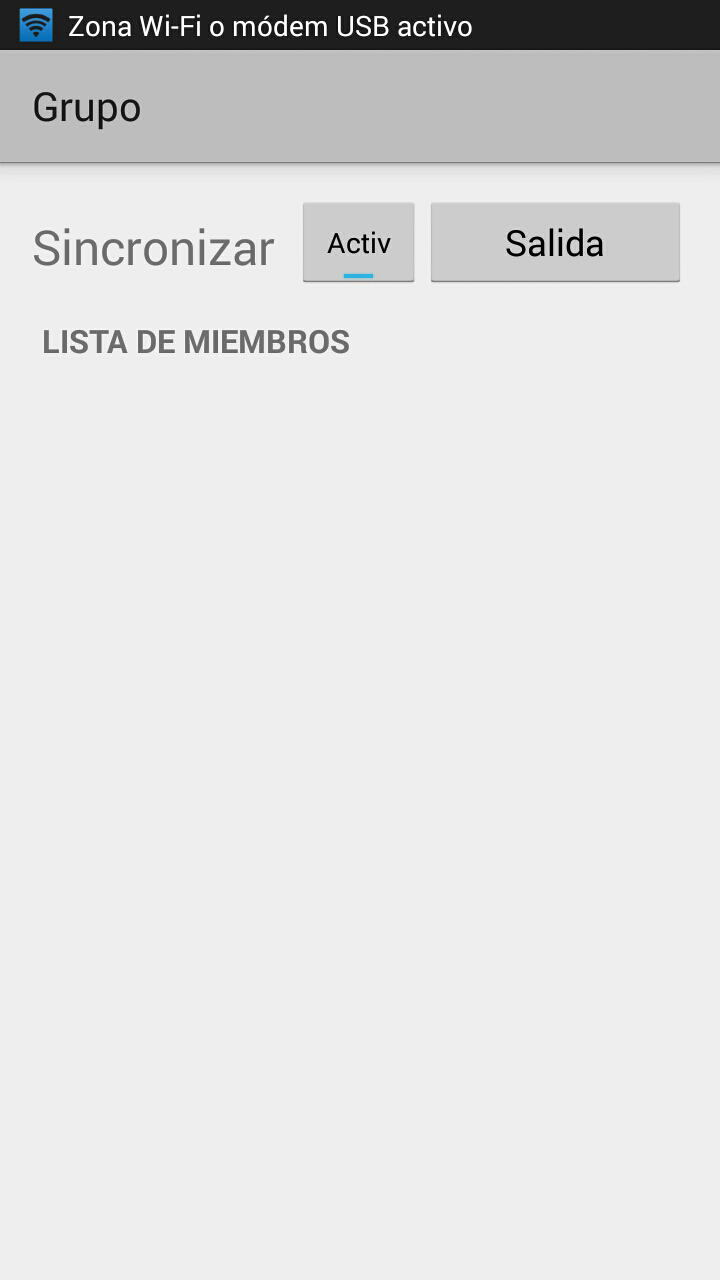
\includegraphics[scale=0.2]{leader_sync}
			\caption{\emph{Hub} del líder}
			\label{figure:Hub}
		\end{center}
	\end{minipage}
\begin{minipage}{.5\textwidth}
	\begin{center}
		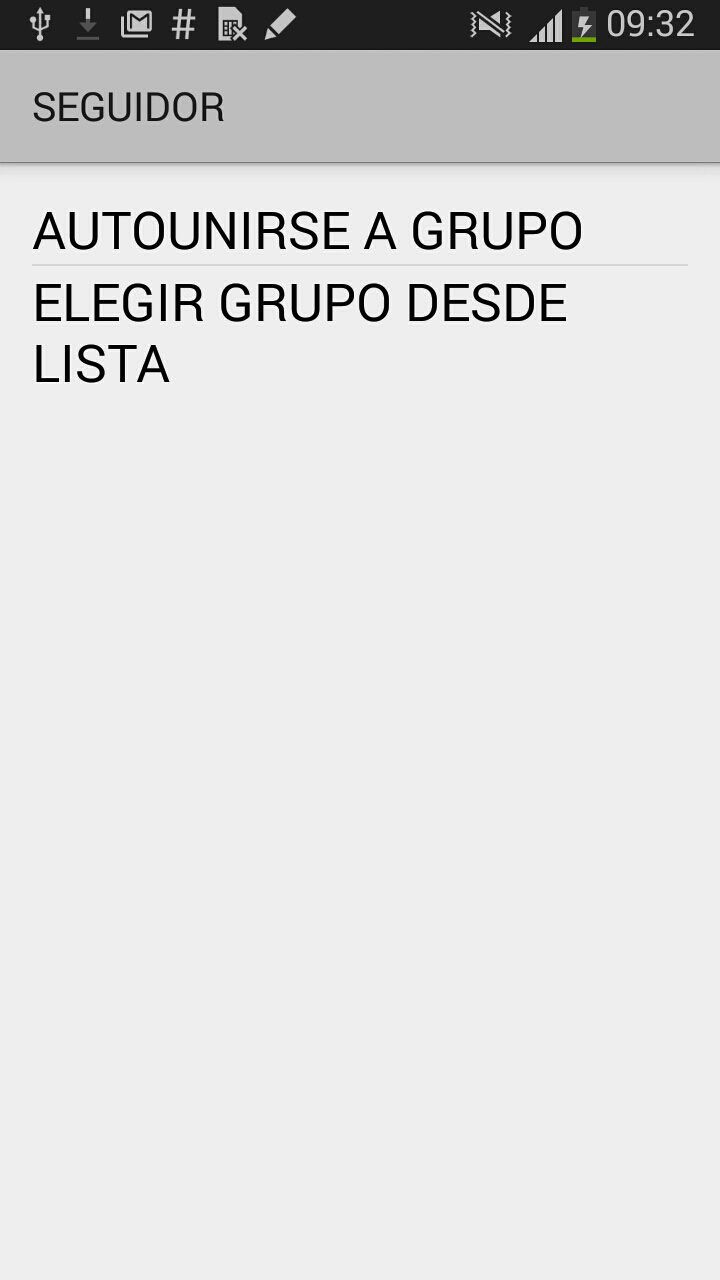
\includegraphics[scale=0.2]{follower_join}
		\caption{Ingreso al grupo del seguidor}
		\label{figure:FollowerJoin}
	\end{center}
\end{minipage}
\end{figure}
		
Para mantener un registro de la ruta que se esta realizando, un controlador mantiene toda la información sobre la salida que se esta realizando. En la figura \ref{figure:DiagramController} se observa la estructura de este controlador, el funcionamiento es como siguiente:
\begin{description}
	\item[AJourney y AGroupJourney] interfáz gráfica que se muestra al usuario (figura \ref{figure:Journey}).
	\begin{figure}[H]
		\begin{center}
			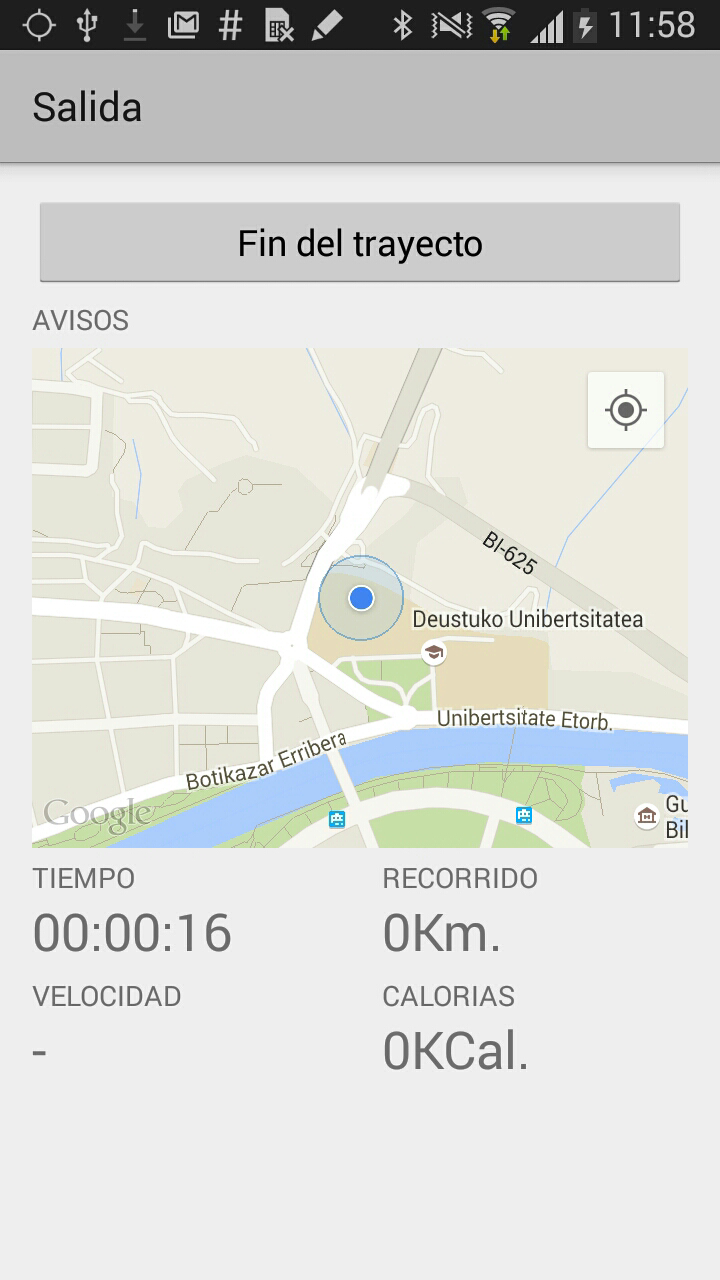
\includegraphics[scale=0.2]{journey}
			\caption{UI de la salida}
			\label{figure:Journey}
		\end{center}
	\end{figure}			
	\item[UIUpdateListener] escuchador de los eventos que se generan en cuanto un mensaje es recibido. Actualizará la interfaz gráfica para mostrar la información al usuario.
	\item[GPSController] encargada de activar el \emph{GPS} y subscribirse a las actualizaciones de posición. Se ha configurado para refrescar la posición cada dos segundos, cuando esto sucede se envía una notificación a la nube con los datos recogidos.
	\item[JourneyController] gestor de la salida. Controla los datos relacionados con la salida: tiempo, distancia recorrida, ruta y calorías quemadas. Permite ser pausada y reanudada.
\end{description}
		
\begin{figure}[H]
	\begin{center}
	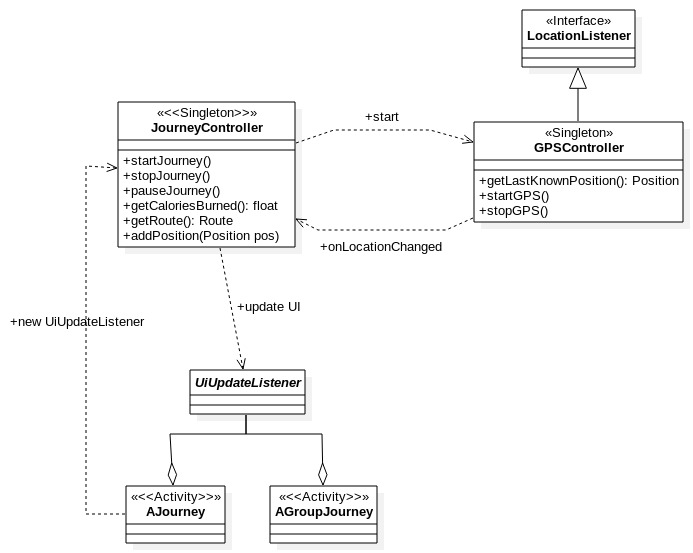
\includegraphics[scale=0.4]{fDiagramJourneyController}
	\caption{Controlador de la salida}
	\label{figure:DiagramController}
	\end{center}
\end{figure}
		
\subsection{Comunicación con la nube}\label{ssection:comunicacion_nube}
Cuando la posición del ciclista es actualizada, se formatean los datos en un objeto JSON y se envían a la nube por medio de un mensaje \emph{HTTP/1.1 POST}. El dominio del servidor es fijo, por lo que siempre se tendrá localizado la dirección de destino [Algoritmo \ref{alg:CyclistSend}]. Cuando el mensaje es recibido por la nube, la aplicación comprobará si el ciclista tiene algún peligro cerca. Si se detecta un vehículo cercano, la aplicación desplegada en la nube contestará con un mensaje de alerta con la información del vehículo detectado y la distancia que les separa.

\begin{listing}
	\begin{minipage}{.4\textwidth}
		\begin{minted}[linenos=true]{java}
HttpClient httpClient;
HttpPost httpPost;
String data;
							
data ="{\"id\":\"" + cyclist.getIdentifier() + "\"," +
  "\"type\"": + "\"cyclist_position\"," +
  "\"latitude\":\"" + cyclist.getPosition().getLatitud() +  "\"," +
  "\"longitude\":\"" + cyclist.getPosition().getLongitud() + "\"," +
  "\"altitude\":\"" + cyclist.getPosition().getAltura() + "\"," +
  "\"heading\":\"" + cyclist.getPosition().getRumbo() + "\"," +
  "\"speed\":\"" + cyclist.getSpeed() + "\"," +
  "\"components\":\"" + cyclist.getPersonas() + "\"," +
  "\"timestamp\":\"" + new Timestamp(new Date().getTime()) + "\"}";
httpClient = new DefaultHttpClient();
httpPost = new HttpPost("http://cloud.mobility.deustotech.eu/cyclist");
httpPost.setEntity(new StringEntity(data));
httpClient.execute(httpPost);
		\end{minted}
	\end{minipage}
	\caption{Envío de peticiones desde la aplicación de ciclistas a la Nube de Ciclistas}\label{alg:CyclistSend}
\end{listing}

Para la recepción de mensajes, la aplicación tiene que pedir un ''token'' de registro único del servidor \emph{GCM} (\emph{Google Cloud Messaging})\footnote{Servicio de mensajería ofrecido por \emph{Google} para enviar y recibir mensajes desde diferentes plataformas.}. Para ello el dispositivo tiene que tener instalado los servicios \emph{Google Play}. Una vez obtiene el ''token'', cuando se envíe un mensaje al servidor se incluirá este identificador dentro del contenido para que la aplicación en el servidor pueda saber a qué dispositivo debe responder. Tras haber realizado la autentificación con los servicios de Google, un escuchador espera a nuevas notificaciones y los procesa una vez han llegado [\ref{figure:DiagramGCM}].
\begin{figure}[h]
	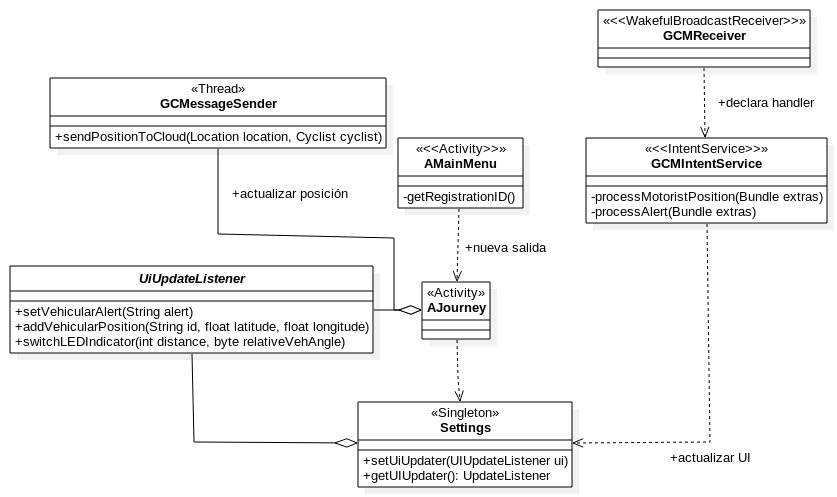
\includegraphics[scale=0.4]{fDiagramGCM}
	\caption{Estructura de la comunicación GCM}
	\label{figure:DiagramGCM}
\end{figure}

\subsection{Comunicación del grupo}\label{ssection:comunicacion_grupo}
Entre los seguidores y el líder se enviarán notificaciones sobre el estado actual de cada nodo (Tabla \ref{table:groupMessages}) a través de del modo \emph{Hub} que tienen los dispositivos; la explicación completa puede encontrarse en la subsección % TODO AÑADIR LA REFERENCIA A LA SUBSECCIÓN

\begin{table}[H]
	\centering
	\caption{Tipo de mensajes en grupo}\label{tab:MensajesGrupo}
	\begin{tabular}{lll}
		\toprule
			\textbf{MENSAJE} & \emph{Descripción} & Campos extra \\
		\midrule
			REGISTER	&	Petición de ingreso de un seguidor al \emph{Hub}. 				& \emph{nombre} 	\\
			ACCEPT		&	Respuesta de aceptación de ingreso de un seguidor al \emph{Hub}. 	& - 				\\
			KICK		&	El administrador echa del \emph{Hub}a un seguidor. 					& - 				\\
			START		&	Notificación de comienzo de la salida.							& - 				\\
			STOP		&	Fin de una salida.								& - 				\\
			PAUSE		&	Notificación de pausa de la salida.								& - 				\\
			RESUME		&	Notificación de reanudado de la salida.							& - 				\\
			ALERT		&	Alerta por vehículo cercano.										& Tabla \ref{tab:CamposMensajePosCiclistaNubeConductores}\\
			MOTORIST\_POSITION & Posición de un vehículo.									& Tabla \ref{tab:CamposMensajePosVehMotNubeConductores}\\
		\bottomrule
	\end{tabular}
\end{table}
Los mensajes son enviados a través del protocolo de transporte \emph{UDP} para que la recepción de mensajes sea lo más rápido posible. Al ser un canal poco fiable se ha implementado una capa para garantizar la recepción del mensaje: cuando un mensaje es enviado, se almacena en un HashTable utilizando como clave la IP del destinatario y un número identificativo del mensaje\footnote{El HashTable solo permite una clave, por lo que se ha creado una clase que calcula un Hash en base a las dos claves con que deseamos identificar el datagrama.}. El receptor mandará un ACK al emisor cuando un mensaje le llegue, y este último eliminará del HashMap el registro previamente almacenado. En caso de que un mensaje no llegue, un \emph{timeout} provocará que el emisor vuelva a enviar el mismo mensaje al receptor; el \emph{timeout} se incrementará al doble cada re-envío. En caso de que un mensaje no sea recibido al quinto intento, se dejará de intentarlo (figura \ref{figure:groupComm}).
		
\begin{figure}[H]
	\begin{center}
		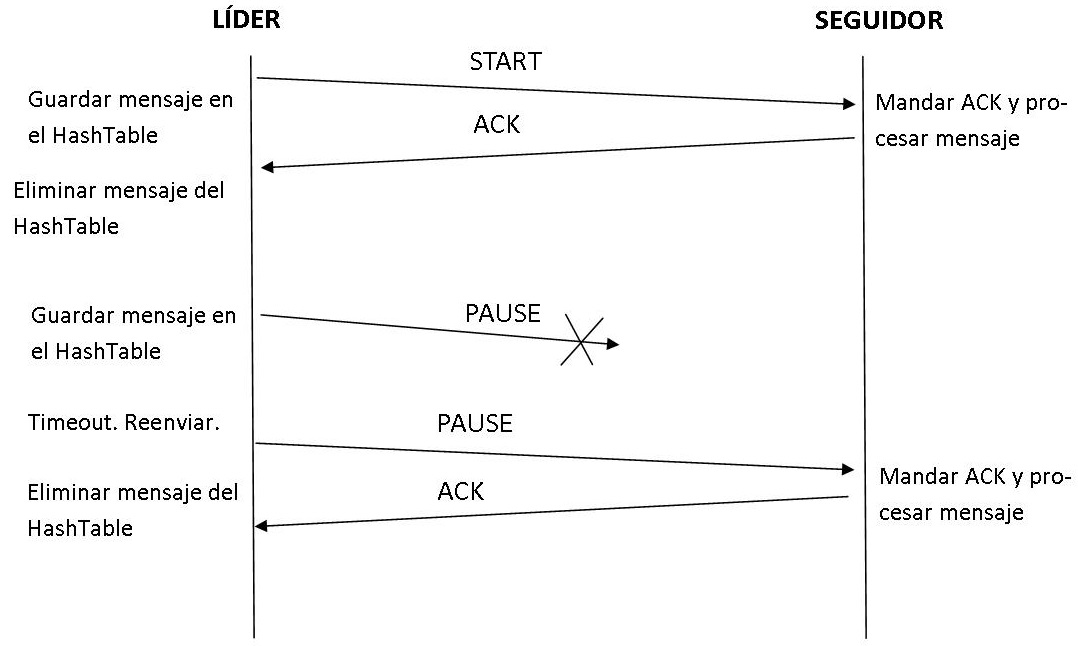
\includegraphics[scale=0.5]{fGroupMessaging}
		\caption{Comunicación líder-seguidor}
		\label{figure:groupComm}
	\end{center}
\end{figure}

\subsection{Casco BLE}\label{ssection:cascoBLE}
El ciclista no puede estar pendiente de los avisos de su Smartphone continuamente, ya que esto puede poner en riesgo su seguridad. Para que el ciclista pueda mantener la vista en la vía y tenga la posibilidad de saber si hay algún vehículo que pueda ponerle en riesgo, se ha integrado una \emph{mota Texas CC2540} en el casco del ciclista conectado a varios LEDs que según un código de colores le informan al ciclista sobre eventos que sean peligrosos. Si por ejemplo hay un vehículo acercándose por el lado izquierdo, un LED amarillo o rojo se encenderá, dependiendo si la distancia es menor de 50 ó 20 metros respectivamente.

Este dispositivo utiliza el estándar BLE para comunicarse con la aplicación móvil mediante cortos mensajes de 8 bytes, los cuales contienen un código hexadecimal que representa la combinación de LEDs que deben encenderse. % %TODO Añadir en el apéndice información sobre BLE

\begin{description}
	\item[Programación de la mota] La mota contiene un pequeño programa escrito en lenguaje C que se encuentra flasheado en su ROM (Read Only Memory). Este programa configura el micro-controlador para actuar como servidor (denominado \emph{Central}), a la espera de ser emparejado y recibir mensajes. Hasta que se sincroniza con un dispositivo, cada 50 mili segundos propaga una señal para que los dispositivos puedan emparejarse. Cuando un dispositivo se conecta, el micro controlador espera a recibir un pequeño mensaje con el código de la señal que le especificará qué LEDs debe encender. Cuando llega el mensaje, si el código recibido es el correcto enciende el LED correspondiente. Para el desarrollo  de este programa se ha trabajado sobre una plantilla, que provee Texas Instrument junto con el dispositivo CC2540, al que se ha añadido el servicio necesario para encender el LED al recibir una señal. En el algoritmo \ref{alg:mota} se explica cómo se ha implementado un nuevo servicio para gestionar los mensajes entrantes.
	
	
	\item[Programación de la app] La aplicación de ciclistas actúa como cliente, por lo que el usuario debe primero emparejarse con el casco para que pueda comenzar a comunicarse con la mota. El proceso de conexión y envío de mensajes consiste:
		\begin{enumerate}
			\item Buscar los servicios Bluetooth disponibles.
			\item Conectar al dispositivo en cuestión.
			\item Descubrir los servicios que ofrece el dispositivo. Esto devolverá varios UUIDs con los servicios que tiene disponibles la mota. Una vez se sabe cuál es el servicio que controla la recepción de mensajes, hay que obtener una referencia. 
			\item Descubrir las características que contiene el servicio. Empleando la referencia del servicio, se pueden obtener uno o varios UUID que representan variables en las que se puede escribir un valor. Aquí es donde se depositará el código de combinación de LEDs que se desea encender [\ref{alg:mota1}].
			\item Escribir sobre la característica que gestiona los LEDs [\ref{alg:mota2}].
		\end{enumerate}
		
		\begin{listing}
			\begin{minipage}{.4\textwidth}
				\begin{minted}[linenos=true]{java}
public void conectarBLE(Device dispositivo) {
  // El primer argumento indica que la propia clase gestionará los eventos,
  // el segundo argumento que se autoconectará al dispositivo, y el tercer
  // argumento a qué dispositivo va a conectarse.
  bluetoothGatt = device.connectGatt(this, false, dispositivo);	
}

public void mandarMensajeBLE(byte msg) {
  // obtener el servicio que contiene la característica que se va a modificar
  servicio = bluetoothGatt.getService(UUID\_SERVICIO);	
  
  // obtener la característica (local)
  caracteristica.getCharacteristic(msg);
  
  // modificar el valor de la característica (local)
  caracteristica.setValor(msg);
  
  // aplicar cambios en el dispositivo remoto
  bluetoothGatt.writeCharacteristic(caracteristica);	
}	
				\end{minted}
			\end{minipage}
		\caption{Envío de mensajes LED desde la aplicación de ciclistas}\label{alg:appciclistasBLE}
	\end{listing}
\end{description}

\begin{table}[H]
	\centering
	\caption{Tabla de la verdad de señales LED}\label{tab:tablaVerdadLED}
	\begin{tabular}{lll}
		\toprule
		\textbf{SEÑAL} & \emph{MNEMÓNICO} & DESCRIPCIÓN \\
		\midrule
		
		0x00    & NONE    & Sin peligro. Apagar los LED \\
		0x01    & AL\_RIGHT & Vehículo a menos de 20 metros por la derecha. Encender luz roja derecha. \\
		0x02    & AL\_LEFT & Vehículo a menos de 20 metros por la izquierda. Encender luz roja izquierda. \\
		0x03    & AL\_BACK & Vehículo a menos de 20 metros por detrás. Ambas luces rojas encendidas. \\
		0x04    & AL\_FRONT & Vehículo a menos de 20 metros por delante. Ambas luces rojas encendidas parpadeando. \\
		0x11    & W\_RIGHT & Vehículo a menos de 50 metros por la derecha. Encender luz amarilla derecha. \\
		0x12    & W\_LEFT & Vehículo a menos de 50 metros por la izquierda. Endernder luz amarilla izquierda. \\
		0x13    & W\_BACK & Vehículo a menos de 50 metros por detrás. Ambas luces amarillas encendidas. \\
		0x14    & W\_FRONT & Vehículo a menos de 50 metros por delante. Ambas luces amarillas parpadeando encendidas.\\
		\bottomrule
	\end{tabular}
\end{table}

\section{Comunicación vehicular}
Los RSU y OBU son los encargados de proveer las posiciones de los vehículos a motor de la \emph{Nube de Conductores}. El OBU se encuentra integrado en el vehículo, y envía a través de \emph{IEEE 802.11p} las posiciones de los vehículos a la RSU. La RSU recoge los datos enviados por la OBU y los retransmite a la nube, al igual que recibe datos de la nube y los retransmite al OBU.

	\subsection{Unidad en carretera}
	Formato por un router que se comunica a través de \emph{IEEE 802.11p}, y un computador conectado tanto al router como a una red LTE. Actúan como puente entre las OBU instaladas en los vehículos y la nube. El RSU escucha y escribe a través de dos canales:
	
	\begin{enumerate}
		\item En el canal LTE recibe los mensajes HTTP/1.1 que provienen de la Nube de Conductores, así como envía las posiciones de los vehículos a la nube. Un Servicio web posibilita la gestión de estos mensajes; el formato es el mismo que el explicado en la sección \ref{ssection:FormatoMensajesNC}.
		
		\item Escucha el canal IEEE 802.11p los mensajes que son enviados por los vehículos, y los redirige a la nube a través de mensajes HTTP/1.1.
	\end{enumerate}
		\subsubsection{Funcionamiento}
		\begin{enumerate}
			\item Se comprueba que el formato del mensaje es correcto. Si no lo es, se descarta.
			\item Lectura del campo \"TYPE\" del mensaje. Dependiendo de su contenido se aplica un proceso diferente: el mensaje puede ser retransmitido a través de Broadcast, se puede mostrar una notificación en un panel informativo en carretera...
		\end{enumerate}
		
		Una propuesta para añadir funciones adicionales consiste en conectar el RSU a elementos informáticos que pueden existir en la carretera, por ejemplo los paneles informativos, y al enviar un mensaje desde la Nube de Conductores a una RSU en concreto se muestra la información deseada.

\subsection{Unidad en el vehículo}
Dentro del ecosistema vehicular existen varias unidades con diferentes papeles: el OBU, el HMI (Human-Machine interface) y la interfaz OpenXC (o tecnología equivalente). Para darse la comunicación con todas las plataformas se depende de la existencia de RSU desplegadas en la carretera.

	\subsubsection{OBU}
	Formado por un router que se comunica a través de IEEE 802.11p, un dispositivo GPS conectado al router, y un computador conectado al router a través de un conector RJ-45. A traves de esta red se reciben mensajes de diferentes RSU que se encuentran desplegadas en la carretera, al igual que se envían mensajes informando sobre la posición del vehículo a través de Broadcast. Su funcionamiento consiste en:
	\begin{itemize}
		\item Obtener la posición del vehículo realizando peticiones al router.
		\item Mandar periódicamente las posiciones a través de broadcast.
		\item Escuchar los mensajes que mandan las RSU.
		\item Ofrecer y proveer al usuario la información de los mensajes a través del HMI.
	\end{itemize}
	
	\subsubsection{Información al usuario}
	Para proveer información al conductor se emplea el HMI, el cual consiste enun ordenador de a bordo que contiene diferentes apps. Adicionalmente, se puede conectar al OBDII (On-Board Diagnostic)\footnote{Se trata del sistema de diagnóstico del vehículo. Provee información sobre el estado de los diferentes subsistemas del vehículo.} a través de un puerto RS 232 para obtener información del vehículo; como por ejemplo, el estado de los neumáticos.
	
	Se ha desarrollado una plaicación conectada por Bluetooth al OBU con la que se muestra al vehículo un mapa con las posiciones de los ciclistas cercanos [Imagen \ref{figure:HMI}]. Cuando un vehículo se acerca a un ciclista o grupo de ciclistas una notificación salta para informar al conductor. Las posiciones de los ciclistas son obtenidas a través de la nube, y almacenadas en el vehículo durante un período de 30 segundos; según llegan las nuevas posiciones desde la nube, se van actualizando. Pasado ese tiempo, los registros que no hayan sido refrescados son eliminados, ya que esto significaría que los nodos han dejado de transmitir.
	
	\begin{figure}[H]
			\begin{center}
				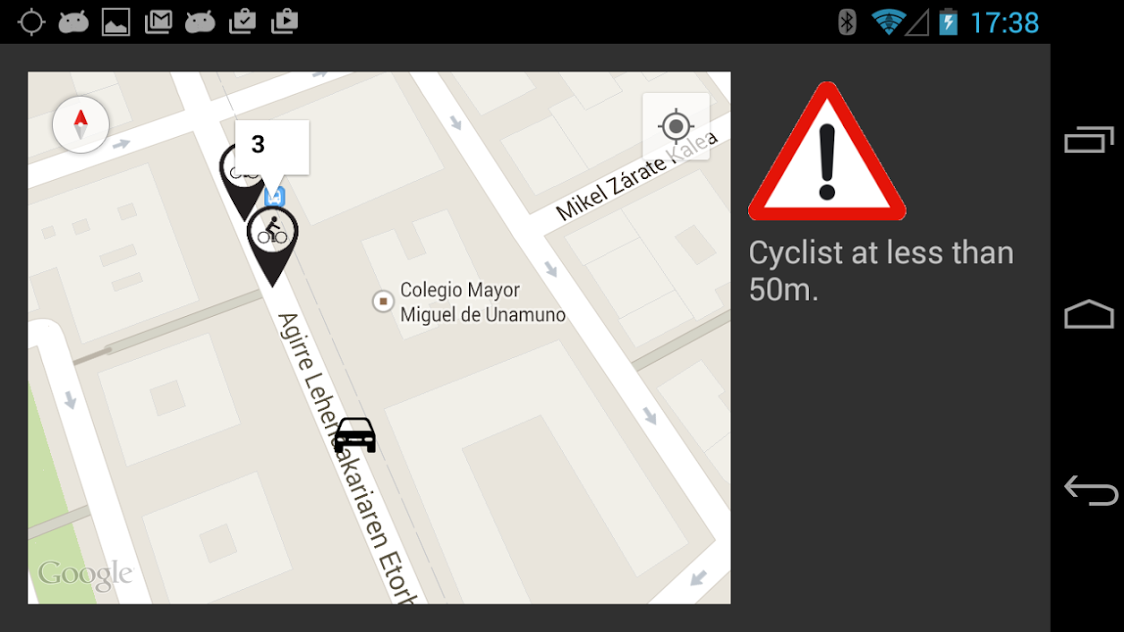
\includegraphics[scale=0.4]{HMI}
				\caption{UI de la aplicación instalada en el HMI}
				\label{figure:HMI}
			\end{center}
	\end{figure}
	
	\subsubsection{Comunicación HMI-OBU}
	Para crear el servidor Bluetooth que envíe los mensajes recibidos por el OBU a la aplicación instalada en el HMI, se ha utilizado la librería Bluecove. En el \ref{alg:puntoAccesoHMI_OBU} se abre un punto de acceso para clientes Bluetooth, y se envían los mensajes que se han recibido en el OBU y deben ser mostrados al usuario.

	\begin{listing}
		\begin{minipage}{.4\textwidth}
			\begin{minted}[linenos=true]{java}
BluetoothServer server;
StreamConnection cnn;
BufferedWriter writer;
final String UUID = "btspp://localhost:432814212fd123e;name=obu";
StreamConnectionNotifier notifier;
					
// 1. Para que el HMI pueda conectarse al OBU la conexión primero se debe hacer
// visible bajo un UUID determinado.
LocalDevice.getLocalDevice().setDiscoverable(DiscoveryAgent.GIAC);
cnn = notifier.acceptAndOpen();					
					
// 2. Se espera a que un cliente se conecte al servicio Bluetooth
writer = new BufferedWriter(new OutputStreamWriter(cnn.openDataOutputStream()));
					
// 3. Una vez conectado, se envían mensajes al cliente en cuanto son recibidos, mediante
// una cola de mensajes
[...]
					
// 4. Se cierra el socket al finalizar la conexión
writer.close();
cnn.close();
			\end{minted}
		\end{minipage}
		\caption{Creación de un punto de acceso Bluetooth en el OBU}\label{alg:puntoAccesoHMI_OBU}
	\end{listing}

